\documentclass{beamer}
%\usetheme{Singapore}
\usepackage{tikz}
\usetikzlibrary{arrows,automata}
\usepackage{multicol}
%\usepackage{pstricks,pst-node,pst-tree}
\usepackage{amssymb,latexsym}
\usepackage{graphicx}
\usepackage{fancyvrb}
\usepackage{hyperref}

\newcommand{\bi}{\begin{itemize}}
\newcommand{\ii}{\item}
\newcommand{\ei}{\end{itemize}}
\newcommand{\Show}[1]{\psshadowbox{#1}}


\newcommand{\grf}[2]{\centerline{\includegraphics[width=#1\textwidth]{#2}}}
\newcommand{\tw}{\textwidth}
\newcommand{\bc}{\begin{columns}}
\newcommand{\ec}{\end{columns}}
\newcommand{\cc}[1]{\column{#1\textwidth}}

\newcommand{\bfr}[1]{\begin{frame}[fragile]\frametitle{{ #1 }}}
\newcommand{\efr}{\end{frame}}

\newcommand{\cola}[1]{\begin{columns}\begin{column}{#1\textwidth}}
\newcommand{\colb}[1]{\end{column}\begin{column}{#1\textwidth}}
\newcommand{\colc}{\end{column}\end{columns}}

\title{Introduction to Theory of Computation}
\author{Chapters 4 and 5, Turing Machines and Decidability}

\RecustomVerbatimEnvironment{Verbatim}{Verbatim}{frame=single}

\newcommand{\pth}[5]{\path (#1) edge node {$\frac{#2}{#3 #4}$} (#5); }
\newcommand{\pthl}[5]{\path (#1) edge [bend left] node {$\frac{#2}{#3 #4}$} (#5); }
\newcommand{\pthr}[5]{\path (#1) edge [bend right] node {$\frac{#2}{#3 #4}$} (#5); }
\newcommand{\pthla}[5]{\path (#1) edge [loop above] node {$\frac{#2}{#3 #4}$} (#5); }
\newcommand{\pthlb}[5]{\path (#1) edge [loop below] node {$\frac{#2}{#3 #4}$} (#5); }
\newcommand{\pthlr}[5]{\path (#1) edge [loop right] node {$\frac{#2}{#3 #4}$} (#5); }
\newcommand{\pthll}[5]{\path (#1) edge [loop left] node {$\frac{#2}{#3 #4}$} (#5); }


\begin{document}
\begin{frame}
\maketitle

\end{frame}

\bfr{Alan Turing}
\begin{multicols}{2}
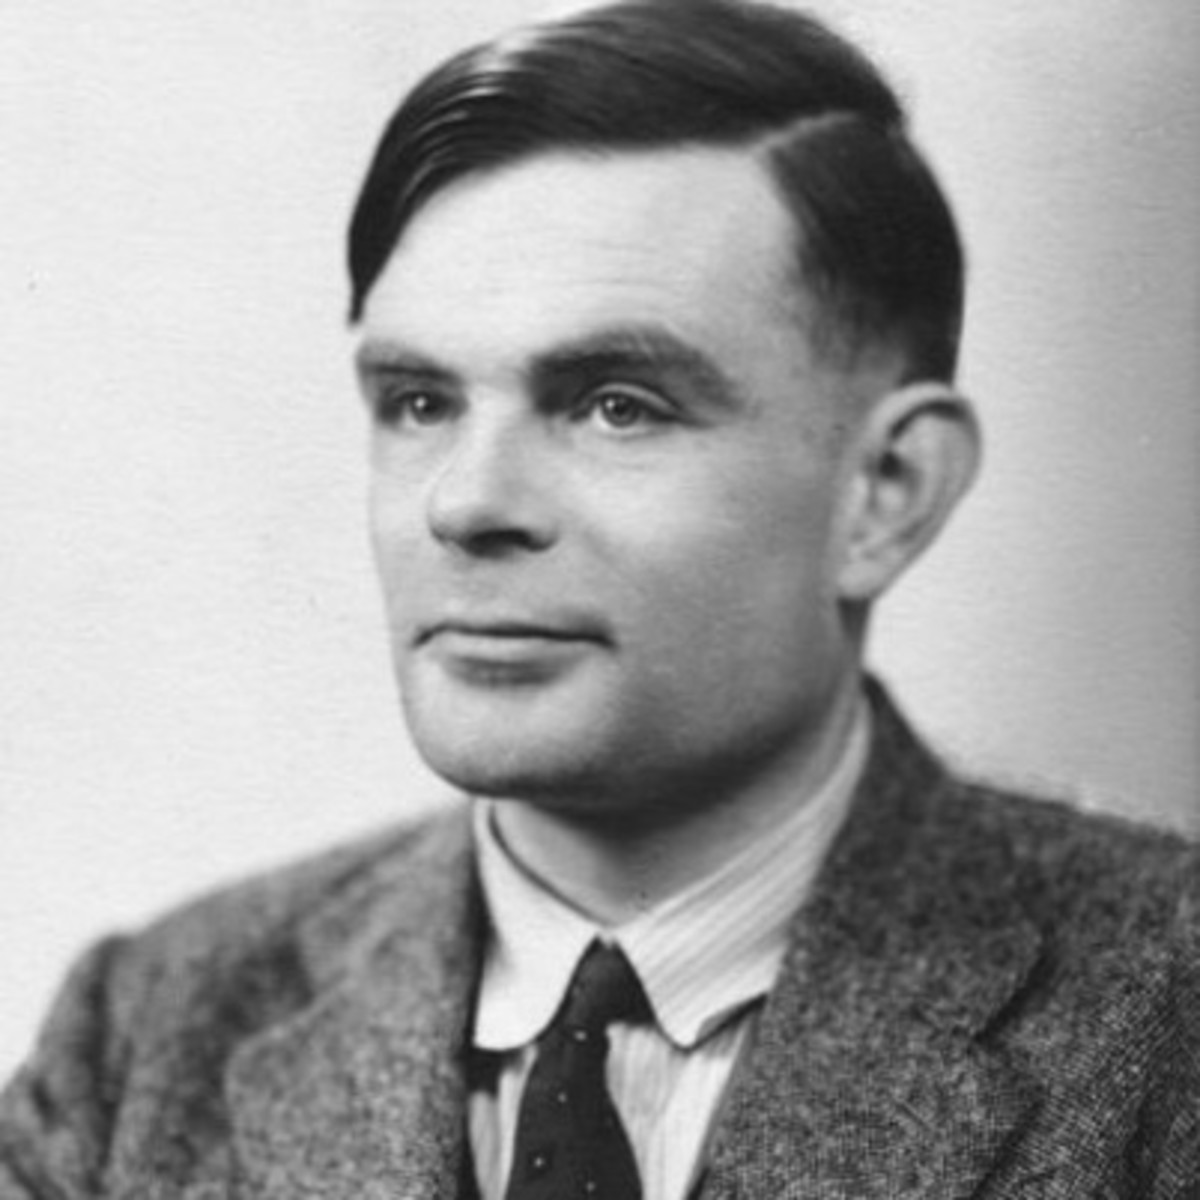
\includegraphics[width=0.5\textwidth]{Turing}
\columnbreak
\begin{itemize}
  \pause
\item Defeated Nazi Enigma code machine in WWII.
  \pause
\item Designed and built one of the first computers.
  \pause
\item Developed philosophy of artificial intelligence.
  \pause
\item Developed theory of computability.
  \pause
\item Invented roundhouse chess.
  \pause
\end{itemize}
\end{multicols}

\begin{itemize}
\item Convicted of homosexuality in 1952.
  \pause
\item Sentenced to chemical castration by synthetic estrogen.
  \pause
\item Committed suicide in 1954, 16 days before 42nd birthday.
\end{itemize}

\end{frame}

\bfr{Turing Machine}
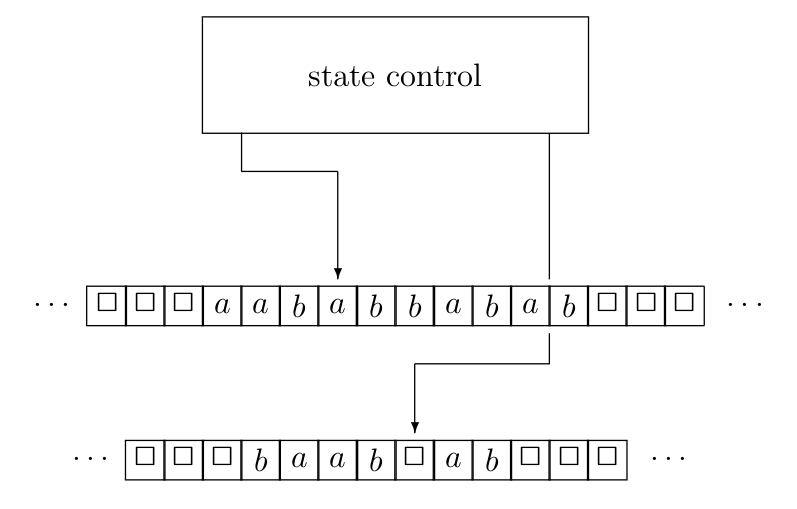
\includegraphics[width=\textwidth]{tm}
\end{frame}

\bfr{Even Palindromes}
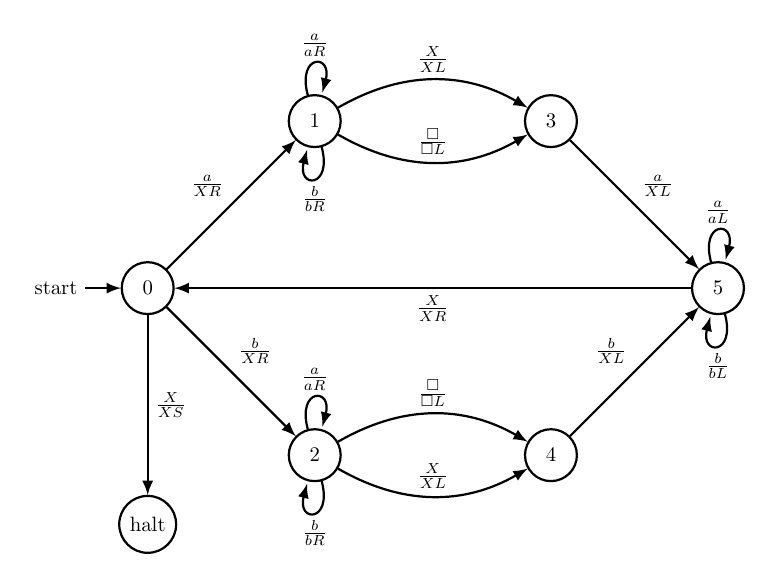
\begin{tikzpicture}[->,>=latex,thick,node distance=4cm,auto,every node/.style={scale=0.75}]
  \node[state,initial] (0) {0};
  \node[state] (1) [above right of=0] {1};
  \node[state] (2) [below right of=0] {2};
  \node[state] (3) [right of=1] {3};
  \node[state] (4) [right of=2] {4};
  \node[state] (5) [below right of=3] {5};
  \node[state] (halt) [below of=0] {halt};
  \path (0) edge node {$\frac{a}{X R}$} (1);
  \path (0) edge node {$\frac{b}{X R}$} (2);
  \path (0) edge node {$\frac{X}{X S}$} (halt);
  \path (1) edge [loop above] node {$\frac{a}{aR}$} (1);
  \path (1) edge [loop below] node {$\frac{b}{bR}$} (1);
  \path (1) edge [bend right] node {$\frac{\square}{\square L}$} (3);
  \path (1) edge [bend left] node {$\frac{X}{X L}$} (3);
  \path (3) edge node {$\frac{a}{X L}$} (5);
  \pthla 2aaR2
  \pthlb 2bbR2
  \pthl 2\square\square L4
  \pthr 2XXL4
  \pth 4bXL5
  \pthla 5aaL5
  \pthlb 5bbL5
  \pth 5XXR0
\end{tikzpicture}

\end{frame}

\bfr{$a^nb^nc^n$}
\begin{tikzpicture}[->,>=latex,thick,node distance=4cm,auto,every node/.style={scale=0.75}]
  \node[state,initial] (0) {0};
  \node[state] (3) [right of=0] {3};
  \node[state] (1) [above of=3] {1};
  \node[state] (2) [right of=1] {2};
  \node[state] (4) [right of=halt] {4};
  \node[state] (halt) [below of=0] {halt};
  \pth 0aXR1
  \pthla 0YYR0
  \pth 0ZZR4
  \pth 0\square\square S{halt}
  \path (1) edge [loop above] node {$\frac{a}{aR}$,$\frac{Y}{YR}$} (1);
  \pth 1bYR2
  \pth 2cZL3
  \path (2) edge [loop above] node {$\frac{b}{bR}$,$\frac{Z}{ZR}$} (2);
  \path (3) edge [loop right] node {$\frac{a}{aL}$,$\frac{b}{bL}$,$\frac{Y}{YL}$,$\frac{Z}{ZL}$} (3);
  \pth 3XXR0
  \pthlr 4ZZR4
  \pth 4\square\square S{halt}
\end{tikzpicture}

\end{frame}

\bfr{Equivalent models:}
\begin{enumerate}
\item One-tape Turing machines.
\item $k$-tape Turing machines.
\item Non-deterministic Turing machines.
\item Java programs.
\item Scheme programs.
\item {\tt C++} programs.
\item ...
\end{enumerate}
\end{frame}

\bfr{A Universal Turing Machine}
\begin{itemize}
\item Any Turing machine $T$ can be described by a string, $\langle T\rangle$.
\item Another Turing machine $U$ can simulate the operation of
  $T$ on input string $w$, when given input
  $\langle T\rangle$ and $w$.
\item A Turing machine, such as $U$,
  that can simulate any other Turing machine is
  called a {\bf Universal Turing Machine}.
\end{itemize}
\end{frame}

\bfr{The Church-Turing Thesis}

{\Large \bf
  Every computational process that is intuitively considered to
  be an algorithm can be converted to a Turing machine.  }
\end{frame}

\bfr{Decidability}

A language $A$ over $\Sigma$
is {\em decidable} if there exists a Turing machine $M$
such that for every string $w\in\Sigma^*$:
\begin{enumerate}
\item If $w\in A$ then $M$, started on $w$, halts in the accept state.
\item If $w\not\in A$ then $M$, started on $w$, halts in the reject state.
\end{enumerate}


\vfill

\begin{itemize}
  \item
I will call a machine like this a {\bf decider} for the language.
\end{itemize}
\end{frame}


\bfr{Enumerability}

A language $A$ over $\Sigma$
is {\em enumerable} if there exists a Turing machine $M$
such that for every string $w\in\Sigma^*$:
\begin{enumerate}
\item If $w\in A$ then $M$, started on $w$, halts in the accept state.
\item If $w\not\in A$ then $M$, started on $w$, either halts in the
  reject state or loops forever.
\end{enumerate}
\vfill
\begin{itemize}
\item
I will call a machine like this a {\bf recognizer} for the language.
\item
A machine that produces each string in a language, one at a time, is
an {\bf enumerator } for the language.
\end{itemize}
\end{frame}



\bfr{Decidable {\em vs.} enumerable}
\begin{itemize}
\item {\bf Decidable} is also called
  \begin{itemize}
  \item {\bf computable}
  \item {\bf recursive}
  \end{itemize}

  \vfill
  
\item {\bf Enumerable} is also called
  \begin{itemize}
  \item {\bf semi-decidable}
  \item {\bf  recognizable}
  \item {\bf recursively enumerable}
  \end{itemize}
\end{itemize}
\end{frame}

\bfr{Enumerator $\Rightarrow$ Recognizer}
If we have an enumerator $M_E$ for a language $L$,\\
we can construct a recognizer $M_R$ for $L$.
\pause
\begin{itemize}
\item $M_R$:
  \begin{itemize}
  \item On input $w$:
    \begin{itemize}
    \item Start running $M_E$, producing series $s_1, s_2, s_3, ...$
    \item If $w=s_i$ for any $i\in\mathbb{N}$, halt with {\bf
      accept}.
    \end{itemize}
  \end{itemize}
\end{itemize}
\end{frame}

\bfr{Recognizer $\Rightarrow$ Enumerator}
If we have a recognizer $M_R$ for a language $L$,\\
we can construct an enumerator $M_E$ for $L$.

\pause
\begin{itemize}
\item $M_E$:
  \begin{itemize}
    \item Generate, one at a time, all possible $s\in\Sigma^*$: $s_1, s_2,
      s_3,...$.
    \item Keep them in a list.
    \item After each string $s_i$ is added to the list, run $M_R$ on
      all strings in the list for $i$ steps.
    \item If any run of $M_R$ accepts a string, output that string and remove
      it from the list.
    \item If any run of $M_R$ rejects a string,  remove
      it from the list.
  \end{itemize}
\end{itemize}
\vfill

This machine will eventually run all possible strings for all possible
number of steps.  Hence, if $M_R$ ever recognizes a string, this
machine will output it.

\end{frame}

\bfr{Describing machines and problems as strings}
\begin{itemize}
\item We assume any machine (DFA, PDA, TM) can be described by a
  string $M$ using some alphabet.
\item The input to any machine is a string $w$ using some alphabet.
\item We can thus describe both a machine $M$ and its input $w$, with a
  pair of strings: $( M,w )$.
\item This pair can be converted to  a single string
  $\langle M,w  \rangle$.
\item  For convenience, we assume   $\langle M,w  \rangle$ is
  encoded in binary.
  \item In general, $\langle x\rangle$ means: encode $x$ as a binary
    string. 
\item We can now define a language $A$ as the set of all strings
  $\langle M,w \rangle$ such that $w\in\mathcal{L}(M)$, the language of $M$.
\end{itemize}
\end{frame}

\bfr{The language $A_{DFA}$ is decidable}
\[
A_{DFA} = \{ \langle M,w\rangle : \mbox{$M$ is a DFA that accepts $w$}\}
\]

Proof?

\pause

\begin{itemize}
\item Given input $\langle M,w\rangle$:
  \begin{itemize}
  \item Run $M$ on $w$.
  \item It must terminate.
  \item If it accepts, accept, else reject.
  \end{itemize}
\end{itemize}
\end{frame}

\bfr{The language $A_{NFA}$ is decidable}
\[
A_{NFA} = \{ \langle M,w\rangle : \mbox{$M$ is a NFA that accepts $w$}\}
\]


Proof?

\pause

\begin{itemize}
\item Given input $\langle M,w\rangle$:
  \begin{itemize}
  \item Convert NFA $M$ to DFA $N$.
  \item This algorithm terminates.
  \item Run $N$ on $w$.
  \item It must terminate.
  \item If it accepts, accept, else reject.
  \end{itemize}
\end{itemize}
\end{frame}

\bfr{The language $A_{CGF}$ is decidable}
\[
A_{CFG} = \{ \langle M,w\rangle : \mbox{$M$ is a CFG that accepts $w$}\}
\]


Proof?

\pause

\begin{itemize}
\item Given input $\langle M,w\rangle$:
  \begin{itemize}
  \item Convert CFG $M$ to Chomsky normal form CFG $N$.
  \item This algorithm terminates.
  \item Generate all derivations of length $2|w|-1$ from $N$.
  \item There are a finite number of these, so it must terminate.
  \item If any derivation yields $w$, accept, else reject.
  \end{itemize}
\end{itemize}
\end{frame}


\bfr{The language $A_{TM}$ is not decidable.}

\[
A_{TM} = \{ \langle M,w\rangle : \mbox{$M$ is a TM that accepts $w$}\}
\]

Proof?\pause\ By contradiction. 

\begin{itemize}
  \item Assume there is a TM $H$ that decides this
    language.
  \item Construct the following TM, $D$:
    
\centerline{
  \fbox{
    \parbox{3in}{
      $D$: On input $\langle M\rangle$:
      \begin{itemize}
      \item Run $H$ on $\langle M, \langle M \rangle\rangle$.
      \item If $H$ accepts, reject, else accept.
      \end{itemize}
    }
  }
}
\item If $H$ accepts $\langle D, \langle D \rangle\rangle$, then
  $D$ rejects $\langle D \rangle$.
  \begin{itemize}
    \item Therefore, by definition $\langle D, \langle D
      \rangle\rangle \not\in A_{TM}$.
  \end{itemize}
\item If $H$ rejects $\langle D, \langle D \rangle\rangle$, then
  $D$ accepts $\langle D \rangle$.
  \begin{itemize}
    \item Therefore, by definition $\langle D, \langle D
      \rangle\rangle \in A_{TM}$.
  \end{itemize}
\item In either case, $H$ does not decide $A_{TM}$.
\end{itemize}

\end{frame}

\bfr{Diagonal argument}
\begin{itemize}
  \item
    Machine $H$ that decides $A_{TM}$ can fill in this table:

\fbox{\parbox{4in}{\[
\begin{array}{cccccccc}
 &  \langle M_0 \rangle &  \langle M_1 \rangle &  \langle M_2 \rangle
 &  \langle M_3 \rangle &  \langle M_4 \rangle &  \langle M_5 \rangle
  & ...\\
  M_0 & \bf accept & accept & accept & reject & accept & reject & ...\\
  M_1 & accept & \bf reject & accept & accept & accept & reject & ...\\
  M_2 & accept & reject & \bf accept & accept & accept & reject & ...\\
  M_3 & accept & accept & reject & \bf reject & accept & accept & ...\\
  M_4 & reject & accept & accept & reject & \bf accept & accept & ...\\
  M_5 & reject & reject & accept & accept & accept & \bf reject & ...\\
  ... &  ... &  ... &  ... &  ... &  ... &  ... &  ... 
\end{array}
\]}}

\item
 $D$ uses $H$ to give the opposite answer on the diagonal.
\item
 $H$ must give the wrong answer somewhere on machine $D$.
  \end{itemize}
\end{frame}


\bfr{The language $A_{TM}$ is enumerable but not decidable.}
\[
A_{TM} = \{ \langle M,w\rangle : \mbox{$M$ is a TM that accepts $w$}\}
\]

Proof?
\pause
\begin{itemize}
\item Given input $\langle M,w\rangle$ :
  \begin{itemize}
  \item Simulate the operation of $M$ on $w$.
  \item If this terminates with accept, accept.
  \end{itemize}
\end{itemize}
      

\end{frame}



\bfr{The language $Halt$ is not decidable.}
\[
Halt = \{ \langle M,w\rangle : \mbox{$M$ is a TM that terminates on $w$}\}
\]

Proof?\pause

By contradiction.  Assume there is a TM $H$ that decides this
language.  Construct the following TM, $Q$:

\centerline{
  \fbox{
    \parbox{3in}{
      $Q$: On input $\langle M\rangle$:
      \begin{itemize}
      \item while $H(\langle M,\langle M \rangle \rangle)$ do end;
      \end{itemize}
    }
  }
}

\begin{itemize}
\item
  What happens if we run $Q$ on itself?
\item
  $Q(\langle Q\rangle) $
  terminates iff   $Q(\langle Q\rangle) $ does not terminate.
  \pause
\item Can also use a diagonal argument.
\end{itemize}

\end{frame}

\bfr{The language $M_a$ is not decidable.}
\[
M_a = \{\langle M \rangle \mid \mathcal{L}(M) = \{a\}\}
\]

Proof?\pause

By contradiction.
\begin{itemize}
\item Suppose TM $A$ decides $M_a$.
\item Construct the following TM, $H$:
  \fbox{
    \parbox{3in}{
  $H$: On input $\langle M, w\rangle$:
      \begin{itemize}
    \item Construct TM $D$:
      \fbox{
        \parbox{2in}{
          $D$: On input $\langle s \rangle$:
          \begin{itemize}
          \item Run $M$ on $w$.
          \item If $s=a$ accept, else reject.
          \end{itemize}
        }
      }
    \item Run $A$ on $D$.  If it accepts, accept, else reject.
    \end{itemize}
  }}\pause
  \item $\mathcal{L}(D) = \{a\}$ iff $M$ halts on $w$.\pause
  \item $H$ decides the language $Halt$. But that's impossible!
\end{itemize}



\end{frame}

\bfr{The language $M_\emptyset$ is not decidable.}
\[
M_\emptyset = \{\langle M \rangle \mid \mathcal{L}(M) = \emptyset\}
\]

Proof?\pause

By contradiction.
\begin{itemize}
\item Suppose TM $A$ decides $M_\emptyset$.
\item Construct the following TM, $H$:
  \fbox{
    \parbox{3in}{
  $H$: On input $\langle M, w\rangle$:
      \begin{itemize}
    \item Construct TM $D$:
      \fbox{
        \parbox{2in}{
          $D$: On input $\langle s \rangle$:
          \begin{itemize}
          \item Run $M$ on $w$.
          \item Accept.
          \end{itemize}
        }
      }
    \item Run $A$ on $D$.  If it accepts, reject, else accept.
    \end{itemize}
  }}\pause
  \item $\mathcal{L}(D) = \emptyset$ iff $M$ does not halt on $w$.\pause
  \item $H$ decides the language $Halt$. But that's impossible!
\end{itemize}



\end{frame}



\bfr{Rice's Theorem}
Let $\mathcal{T}$ be the set of all binary encoded TMs.

Let $\mathcal{P}$ be a subset of $\mathcal{T}$ such that
\begin{enumerate}
\item $\mathcal{P}\not=\emptyset$
\item $\mathcal{P}\not=\mathcal{T}$
\item If $L(M_1) = L(M_2)$, then either both or neither is in $\mathcal{P}$.
\end{enumerate}
Then $\mathcal{P}$ is undecidable.
\end{frame}

\bfr{Rice's Theorem Examples}
\begin{enumerate}
  \item $\{\langle M\rangle\mid \mbox{$M$ accepts only inputs in the language $a^*b^*$}\}$
\item  $\{\langle M\rangle\mid \mbox{$M$ accepts only input of length $n^2$}\}$
\item  $\{\langle M\rangle\mid \mbox{$M$ accepts only input of length $k$}\}$
\item $\{\langle  M\rangle\mid \mbox{$M$ accepts all inputs}\}$
\item $\{\langle  M\rangle\mid \mbox{$M$ does not accept all inputs}\}$
\item $\{\langle  M\rangle\mid \mbox{$M$ accepts some input}\}$
\item $\{\langle  M\rangle\mid \mbox{$M$ does not accept any input}\}$
\end{enumerate}

None of these is decideable.

\end{frame}

\bfr{Hilbert's 10th problem is enumerable but not decidable}
\begin{eqnarray*}
Hilbert = \{\langle p \rangle &:& \mbox{$p$ is a polynomial with integer
  coefficients}\\ &&\mbox{that has an integral root}\}
\end{eqnarray*}

\vfill

\[
15x^3y^2 + 12xy^2z^3 - 17x^9y^2z = 0
\]
\vfill

\hfill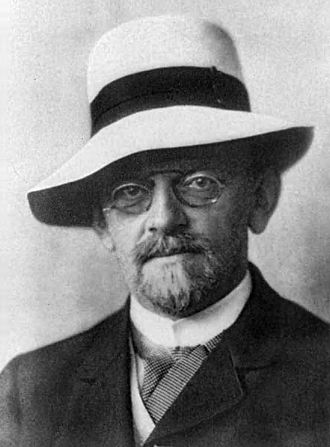
\includegraphics[scale=0.25]{Hilbert.jpg}
\end{frame}

\bfr{Post Correspondence Problem is enumerable but not decidable}
\begin{itemize}
\item
  Given a finite set of dominoes with strings on the top and the bottom,
and an unlimited supply of each domino, does there exist a sequence of
these dominoes such that the string at the top matches the string at
the bottom?
\item
For example, given the set of three dominos:

\begin{center}
  \begin{tabular}{|c|c|c|}\hline
  a & ab & bba \\\hline
  baa & aa & bb \\\hline
  \end{tabular}
\end{center}
\item
We can find a sequence:

\begin{center}
  \begin{tabular}{|c|c|c|c|}\hline
    bba & ab & bba & a \\\hline
    bb & aa & bb & baa \\\hline
  \end{tabular}
\end{center}
\item
Where the top and bottom rows are both: bbaabbbaa
\end{itemize}

\end{frame}

\bfr{Uncomputable real number}

\begin{itemize}
\item A {\em computable real number} is one for which there is a
  Turing machine which, given $n$ on its initial tape, terminates
  with the $n$th digit of the decimal expansion of that
  number encoded on its tape.
  \pause
\item
  All possible Turing machines can be enumerated, since each is
  represented by a unique string.  Let the $i$th Turing machine be
  denoted by $T_i$.
  \pause

\bigskip
\item  
  Let $x$ be the real number between 0 and 1 with the following decimal
  expansion:

  The $i$th digit of $x$ is 1 if $\mathcal{L}(T_I) = \emptyset$,
  otherwise 0.

  \pause
\bigskip
  
  \item $x$ cannot be computable, because its solution would solve the
    halting problem (see above).
\end{itemize}

\end{frame}

\bfr{A language such that both $A$ and $\overline{A}$ are not
  enumerable.}

\begin{align*}
EQ_{TM} &= \{\langle M_1, M_2\rangle:
\mathcal{L}(M_1) = \mathcal{L}(M_2) \}
\end{align*}
\end{frame}

\bfr{$EQ_{TM}$ is not enumerable}
$EQ_{TM} = \{\langle M_1, M_2\rangle:
\mathcal{L}(M_1) = \mathcal{L}(M_2) \}$
\begin{itemize}
\item Suppose $EQ_{TM}$ is recognizable by TM $M_=$.
\item
  Recall that $\overline{Halt}$ is not recognizable.
\item
  For any $M$ and $w$, define the following TM:
  \fbox{
    \parbox{3in}{
      $M_{Mw}$: on input $s$:
      \begin{itemize}
      \item Run $M$ on $w$.
      \item Accept
      \end{itemize}
  }}
\item Also define:
  
  \fbox{
    \parbox{3in}{
      $M_{\emptyset}$: on input $s$, reject.
  }}
  \fbox{
    \parbox{3in}{
      $M_{\Sigma^*}$: on input $s$, accept.
  }}

\item Run $M_=$ on $\langle M_\emptyset, M_{Mw}\rangle$.
  \begin{itemize}
\item This accepts iff $\langle M,w\rangle\in\overline{Halt}$.
\item Therefore it is a recognizer for $\overline{Halt}$.
  \end{itemize}

\end{itemize}


\end{frame}

\bfr{$\overline{EQ_{TM}}$ is not enumerable}
$\overline{EQ_{TM}} = \{\langle M_1, M_2\rangle:
\mathcal{L}(M_1) \not= \mathcal{L}(M_2) \}$
\begin{itemize}
\item Suppose $\overline{EQ_{TM}}$ is recognizable by TM $M_{\neq}$.
\item
  Recall that $\overline{Halt}$ is not recognizable.
\item
  For any $M$ and $w$, define the following TM:
  \fbox{
    \parbox{3in}{
      $M_{Mw}$: on input $s$:
      \begin{itemize}
      \item Run $M$ on $w$.
      \item Accept
      \end{itemize}
  }}
\item Also define:
  
  \fbox{
    \parbox{3in}{
      $M_{\emptyset}$: on input $s$, reject.
  }}
  \fbox{
    \parbox{3in}{
      $M_{\Sigma^*}$: on input $s$, accept.
  }}

\item Run $M_{\neq}$ on $\langle M_{\Sigma^*}, M_{Mw}\rangle$.
  \begin{itemize}
\item This accepts iff $\langle M,w\rangle\in\overline{Halt}$.
\item Therefore it is a recognizer for $\overline{Halt}$.
  \end{itemize}

\end{itemize}


\end{frame}


\bfr{Busy beavers are not enumerable} The $n$th busy beaver number is
the largest (finite) number of 1s that can be output by a Turing
machine with $n$ states when started on a blank tape.
\end{frame}


\bfr{2 State Busy Beaver: four 1s}
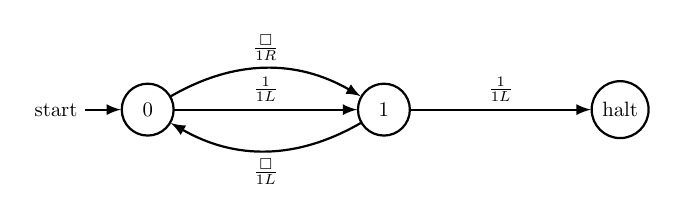
\begin{tikzpicture}[->,>=latex,thick,node distance=4cm,auto,every node/.style={scale=0.75}]
  \node[state,initial] (0) {0};
  \node[state] (1) [right of =0] {1};
  \node[state] (halt) [right of=1] {halt};
  \pthl 0\square 1R1
  \pth 011L1
  \path (1) edge [bend left] node {$\frac{\square}{1L}$} (0);
  \path (1) edge  node {$\frac{1}{1L}$} (halt);
\end{tikzpicture}
 
\end{frame}


\bfr{3 State Busy Beaver: six 1s }
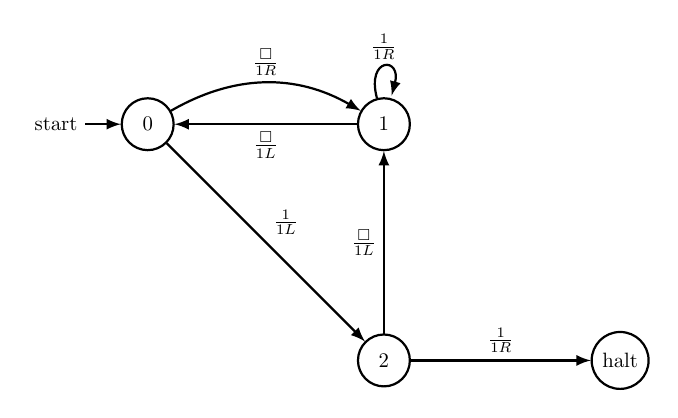
\begin{tikzpicture}[->,>=latex,thick,node distance=4cm,auto,every node/.style={scale=0.75}]
  \node[state,initial] (0) {0};
  \node[state] (1) [right of =0] {1};
  \node[state] (2) [below of =1] {2};
  \node[state] (halt) [right of=2] {halt};
  \pthl 0\square 1R1
  \pth 011L2
  \pth 1\square 1L0
  \pthla 111R1
  \pth 2\square 1L1
  \pth 211R{halt}
\end{tikzpicture}
 
\end{frame}

\bfr{4 State Busy Beaver: thirteen 1s}
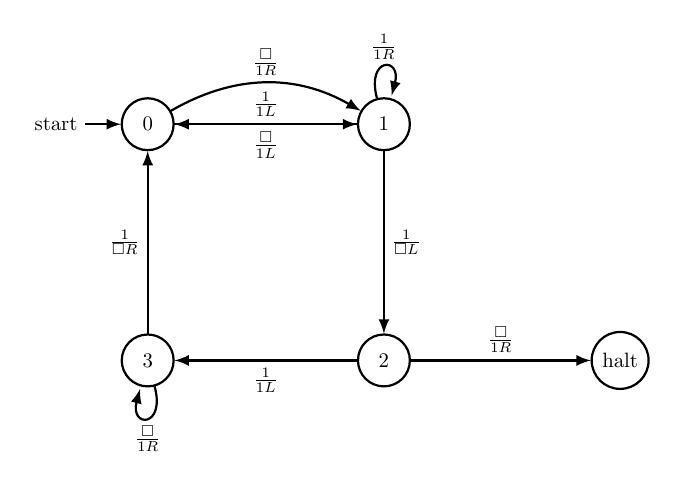
\begin{tikzpicture}[->,>=latex,thick,node distance=4cm,auto,every node/.style={scale=0.75}]
  \node[state,initial] (0) {0};
  \node[state] (1) [right of =0] {1};
  \node[state] (2) [below of =1] {2};
  \node[state] (3) [below of =0] {3};
  \node[state] (halt) [right of=2] {halt};
  \pthl 0\square 1R1
  \pth 011L1
  \pth 1\square 1L0
  \pthla 111R1
  \pth 11\square L2
  \pth 2\square 1R{halt}
  \pth 211L3
  \pthlb 3\square 1R3
  \pth 31\square R0
\end{tikzpicture}
 
\end{frame}


\bfr{5 State Busy Beaver (?): 4098 1s}
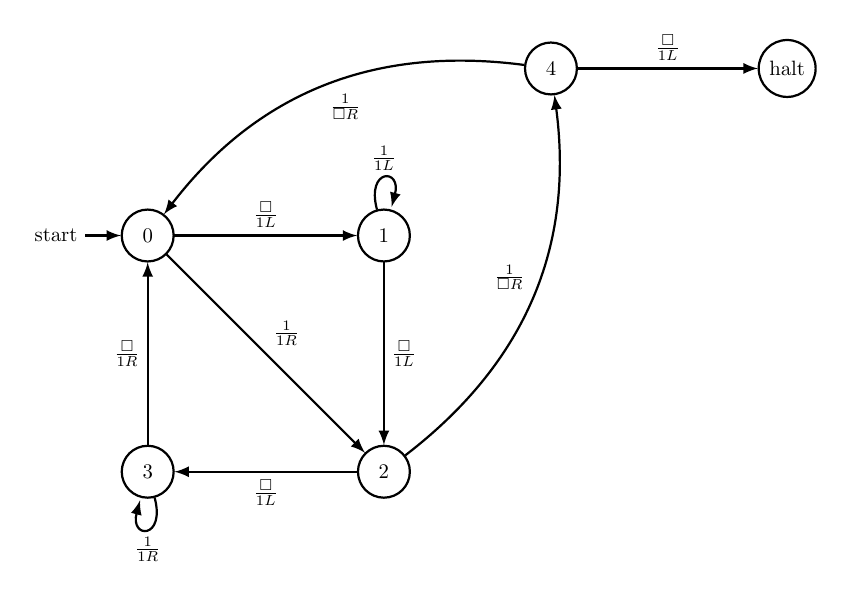
\begin{tikzpicture}[->,>=latex,thick,node distance=4cm,auto,every node/.style={scale=0.75}]
  \node[state,initial] (0) {0};
  \node[state] (1) [right of =0] {1};
  \node[state] (3) [below of =0] {3};
  \node[state] (2) [right of=3] {2};
  \node[state] (4) [above right of=1] {4};
  \node[state] (halt) [right of=4] {halt};
  \pth 0\square 1L1
  \pth 011R2
  \pth 1\square 1L2
  \pthla 111L1
  \pth 2\square 1L3
  \pthr 21\square R4
  \pth 3\square 1R0
  \pthlb 311R3
  \pth 4\square 1L{halt}
  \pthr 41\square R0
\end{tikzpicture}
 
\end{frame}

\bfr{Current Busy Beaver Records}
{\Large
\begin{align*}
  bb(2) &= 4\\
  bb(3) &= 6\\
  bb(4) &= 13\\
  bb(5) &\geq 4098 & \mbox{discovered in 1989}\\
  bb(6) &\geq 3.515 \times 10^{18 267} &\mbox{discovered in 2010}\\
  bb(7) &\geq 10^{10^{10^{10^{18 705 353}}}} &\mbox{actually, much bigger}
\end{align*}
}
\vfill
Note: there are about $10^{80}$ atoms in the universe!
\end{frame}


\bfr{Proof Busy Beaver function is not enumerable}

Proof by contradiction.

\begin{itemize}
\item
Let $bb(n)$ be the largest (finite) number of 1's output by a Turing Machine
with $n$ states.
\item
Suppose there is a Turing Machine $M_{bb}$ that computes $bb(n)$, that is,
starting with $n$ on the tape, the machine halts with $bb(n)$ on the tape.

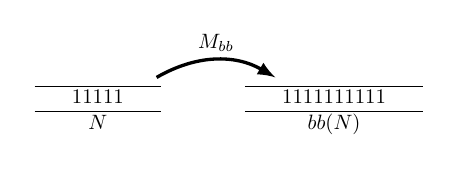
\begin{tikzpicture}[->,>=latex,very thick,node distance=4cm,auto,every node/.style={scale=0.75}]
  \node (1) {
    \begin{tabular}{ccc}\hline
      & 11111 & \\\hline
      & $N$ & \\
    \end{tabular}
  };
  \node (2) [right of=1] {
    \begin{tabular}{ccc}\hline
      & 1111111111 & \\\hline
      & $bb(N)$ & \\
    \end{tabular}
    };
  \path (1) edge [bend left] node {$M_{bb}$} (2);
  \end{tikzpicture}

\item Note: this is a new use of TMs, computing a function
  from input to output, not recognizing a language.
\end{itemize}
\end{frame}

\bfr{Busy Beaver proof}
\begin{itemize}

\item
Let $g(n) = bb(2n)$.  We can build a TM for $g$ by starting with
a machine that doubles the input, and then runs the machine  $M_{bb}$.

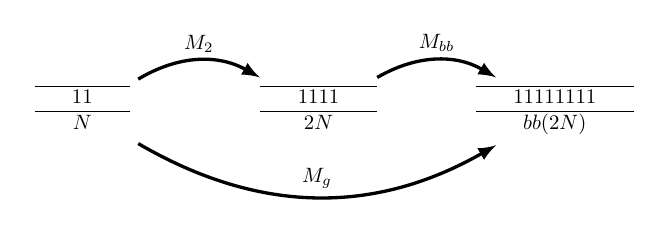
\begin{tikzpicture}[->,>=latex,very thick,node distance=4cm,auto,every node/.style={scale=0.75}]
  \node (3) {
    \begin{tabular}{ccc}\hline
      & 11 & \\\hline
      & $N$ & \\
    \end{tabular}
  };
  \node (4) [right of = 3] {
    \begin{tabular}{ccc}\hline
      & 1111 & \\\hline
      & $2N$ & \\
    \end{tabular}
  };
  \node (5) [right of=4] {
    \begin{tabular}{ccc}\hline
      & 11111111 & \\\hline
      & $bb(2N)$ & \\
    \end{tabular}
    };
  \path (3) edge [bend left] node {$M_{2}$} (4);
  \path (4) edge [bend left] node {$M_{bb}$} (5);
  \path (3) edge [bend right] node {$M_g$} (5);
  \end{tikzpicture}

\item
Suppose the machine for $g$, $M_g$  has $k$ states.

\end{itemize}
\end{frame}

\bfr{Busy Beaver proof}

\begin{itemize}
\item
  Build a machine $M_{2k}$ with $2k$ states that does nothing but put
  $2k$ 1s on a blank tape.
  \item Now build a machine $M_{D}$
  that starts by putting $2k$ 1's on the tape, and then runs the $M_g$
  machine.

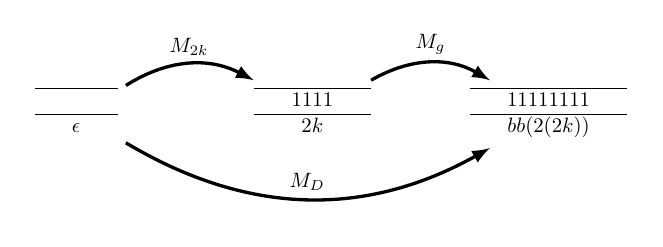
\begin{tikzpicture}[->,>=latex,very thick,node distance=4cm,auto,every node/.style={scale=0.75}]
  \node (6) {
    \begin{tabular}{ccc}\hline
      &  & \\\hline
      & $\epsilon$ & \\
    \end{tabular}
  };
  \node (7) [right of = 6] {
    \begin{tabular}{ccc}\hline
      & 1111 & \\\hline
      & $2k$ & \\
    \end{tabular}
  };
  \node (8) [right of=7] {
    \begin{tabular}{ccc}\hline
      & 11111111 & \\\hline
      & $bb(2(2k))$ & \\
    \end{tabular}
    };
  \path (6) edge [bend left] node {$M_{2k}$} (7);
  \path (7) edge [bend left] node {$M_g$} (8);
  \path (6) edge [bend right] node {$M_{D}$} (8);
  \end{tikzpicture}
\item $M_{D}$ can be built with $3k$ states.
\item The output of $M_{D}$ is $g(2k) = bb(2(2k)) = bb(4k)$ 1s.
\item Do you see the problem?
\end{itemize}
\end{frame}


\bfr{An Old Philosophical Problem}

\centerline{\Large This sentence is false.}

\end{frame}

\bfr{Quine's Paradox}

{\large
  "Yields falsehood when preceded by its quotation"\\
  yields falsehood when preceded by its quotation.
}

\end{frame}

\bfr{Self Reproducing Sentences}

{\large
  Print two copies of the following, the second one in quotes:\\
  "Print two copies of the following, the second one in quotes:"
}
\end{frame}

\bfr{Self Reproducing Programs:  ``Quines''}
\begin{Verbatim}
(define data "Put the program below here,
so long as it doesn't have any strings in it.")
(define (display-as-data data)
  (display (integer->char 40))
  (display 'define)
  (display (integer->char 32))
  (display 'data)
  (display (integer->char 32))
  (display (integer->char 34))
  (display data)
  (display (integer->char 34))
  (display (integer->char 41))
  (newline))
(display-as-data data)
(display data)
\end{Verbatim}
\end{frame}

\bfr{The Recursion Theorem}

Let $T$ be a Turing machine that computes a function
\[
t : \Sigma^*\times \Sigma^* \rightarrow \Sigma^*
\]
There is a Turing machine $R$ that computes a function
\[
r : \Sigma^* \rightarrow \Sigma^*
\]
where, for every $w\in\Sigma^*$,
\[
r(w) = t(w, \langle R \rangle)
\]
\vfill
\pause
\begin{itemize}
\item In other words, given any computation with
  two inputs, we can assume that it is given only one input
  and obtains a description of itself for the second input.
\end{itemize}

\end{frame}

\bfr{The language $A_{TM}$ is not decidable:  EASY PROOF!}
\[
A_{TM} = \{ \langle M,w\rangle : \mbox{$M$ is a TM that accepts $w$}\}
\]

Proof?\pause\ By contradiction. 

\begin{itemize}
  \item Assume there is a TM $H$ that decides this
    language.
  \item Construct the following TM, $B$:

\centerline{
  \fbox{
    \parbox{3in}{
      $B$: On input $\langle w\rangle$:
      \begin{itemize}
      \item Obtain own description, $\langle B \rangle$.
      \item Run $H$ on $\langle B,w\rangle$.
      \item If $H$ accepts, reject, else accept.
      \end{itemize}
    }
  }
}
\item Running $B$ on input $w$ does the opposite of what $H$ says.
\item Therefore, $H$ is wrong about $B$.
\item $H$ does not decide $A_{TM}$.
\end{itemize}

\end{frame}

\end{document}

